\begin{figure}[H]
\centering
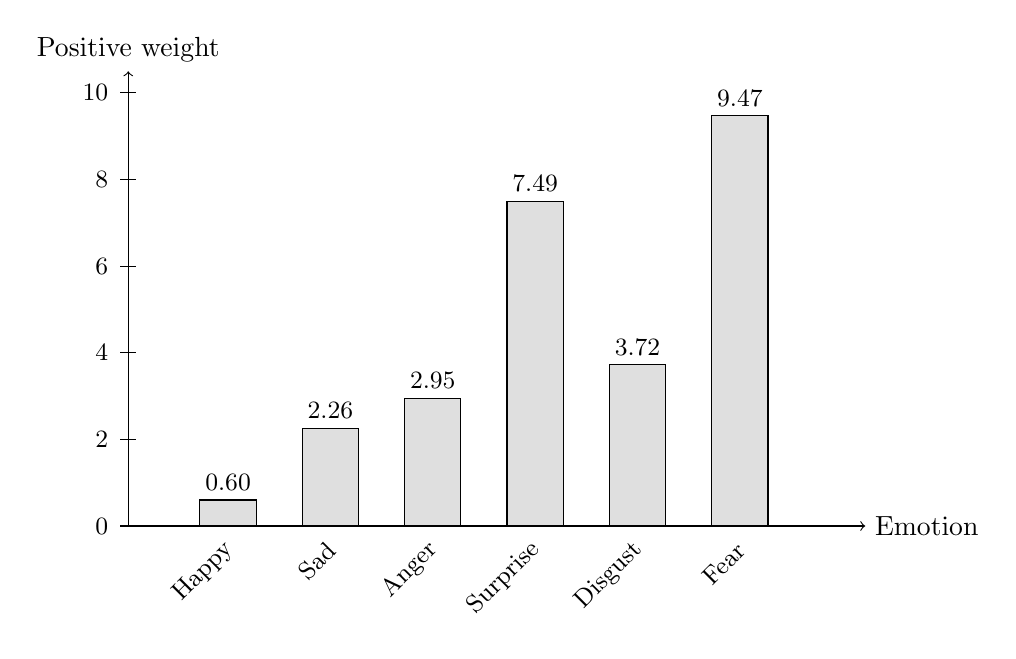
\begin{tikzpicture}[
    x=1.3cm,
    y=0.55cm
]

% Axes
\draw[->] (0,0) -- (7.2,0) node[right] {Emotion};
\draw[->] (0,0) -- (0,10.5) node[above] {Positive weight};

% Y ticks
\foreach \y in {0,2,4,6,8,10} {
    \draw (-0.08,\y) -- (0.08,\y);
    \node[left] at (-0.1,\y) {\small \y};
}

% Bars
\foreach \x/\h/\name in {
    0.7/0.60/Happy,
    1.7/2.26/Sad,
    2.7/2.95/Anger,
    3.7/7.49/Surprise,
    4.7/3.72/Disgust,
    5.7/9.47/Fear
} {
    \draw[fill=gray!25] (\x,0) rectangle +(0.55,\h);
    \node[above, font=\small] at (\x+0.275,\h) {\h};
    \node[rotate=45, anchor=east, font=\small] at (\x+0.35,-0.3) {\name};
}

\end{tikzpicture}
\caption{Class-specific positive weights used in BCEWithLogitsLoss.}
\label{fig:positive_weights}
\end{figure}